\chapter[Event Simulation and Object Reconstruction]{Event Simulation and \protect\\Object Reconstruction}
\label{ch:evSimObjReco}
\epigraph{\emph{Nature isn't classical, dammit, and if you want to make a simulation of nature, you'd better make it quantum mechanical, and by golly it's a wonderful problem, because it doesn't look so easy.}} {Richard P. Feynman}

	The \ac{ATLAS} software framework Athena~\cite{TDR2005}, which is based on the Gaudi~\cite{Gaudi2000} framework developed by \ac{LHCb}~\cite{LHCb2008}, is used to reconstruct physics objects to be used by analysers, as the data collected and recorded by the \ac{ATLAS} detector requires processing. The Athena framework is capable of dealing with various aspects of the experiment software, \eg\ triggering or the processing of simulated data. Custom softwares, in particular \ac{MC} simulations, are used to simulate physics events used to model background and signal process. These are produced through different stages, as shown in Figure~\ref{fig:workflow}, the last of which produces an output with an analyser-friendly format. 

	In this chapter the stages will be briefly explained as it follows: Event Generation (Section~\ref{sec:evGen}) and the Detector Simulation (Section~\ref{subsec:detSim}). The reconstruction of physics objects\footnote{A set of criteria needs to be applied in order to reconstruct the detected object as an ``electron'', ``photon'', ``muon'', ``jet'', etc.}, in both collected data and simulated \ac{MC} events, will be described in Section~\ref{sec:objReco}. Finally, a set of selection criteria are applied to reconstructed objects to identify those suitable for use in analysis, as detailed in Section~\ref{sec:objSel}.

	\begin{figure}
		\centering
		\includegraphics[width=.75\textwidth]{MCobj/flow}
		\caption{\label{fig:workflow} Illustration of the different stages of the workflow needed to produce analysable simulated and collected data outputs. The white boxes represent the processes, and their outputs are shown in black balloons: \ac{RDO}, \ac{ESD}, and the final product, \ac{AOD}. The green `AtlFast' box represents the alternative simulation method \textsc{Atlfast}~\cite{Lukas2012}, discussed in Section~\ref{subsec:detSim}. Finally, the blue box shows the stage at which the actual \ac{ATLAS} data events begin processings.}
	\end{figure}



	\section{Generation of a MC-simulated event}
	\label{sec:evGen}

		\ac{MC} event generators~\cite{Buckley:2011ms} are extensively used in particle physics to simulate \ac{SM} and \ac{BSM} physics processes. A combination of perturbative and phenomenological calculations, to produce randomly distributed physics events, of a given type, with stable final state particles, is employed. As already mentioned in Chapter~\ref{ch:detector}, The \ac{ATLAS} detector collects \pp- and heavy-ion-collisions data. When two protons collide at such high energy in the center of mass, the collision essentially occurs between the nucleon constituents: partons\footnote{``\emph{Feynman~\cite{PhysRevLett.23.1415} interpreted the Bjorken scaling as the point-like nature of the nucleon's constituents when they were incoherently scattered by the incident electron. Feynman named the point-like constituents partons. This is the parton model.}''(taken from~\cite{Yan:2014kna})}. Three valence quarks (uud), the gluons mediating the strong interactions between the valence quarks, and the sea quarks produced in virtual \qqbar\ pairs due to interacting gluons, are included in the partons. Figure~\ref{fig:DIS} shows one of these interactions which are known as \ac{DIS} processes, simply because the substructure of the proton is probed, therefore \emph{deep}, by an incoming particle, in this case a proton, whose momentum is not conserved in the process, therefore \emph{inelastic}.

		\begin{figure}[!htb]
			\centering
			\includegraphics[width=.5\textwidth]{MCobj/ppcollision}
			\caption{\label{fig:DIS} Example of a \pp\ \ac{DIS} event.}
		\end{figure}

		An important yet simplifying dimensionless physical quantity is the Bjorken scaling~\cite{PhysRev.179.1547}, which represents the fraction, $x$, of the proton momentum carried by an interacting parton. The measure of momentum transfer, $Q^2$, in such events, is related to the momentum transferred by the exchanged boson, $q$, by $Q^2 = -q^2$. \ac{PDFs} are used to describe mathematically the parton content of the colliding protons in order to model their interaction.  

		The \pp\ scattering at the \ac{LHC} can be categorised in processes such as \emph{hard}, which can be described with perturbation theory, or \emph{soft}, which involve non-perturbative \ac{QCD} effects. Tipically, a \pp\ collision involves a hard scattering process between two partons, one for each proton, and a certain number of soft processes, such as \ac{ISR}, \ac{FSR}, and \ac{UE}. The \ac{ISR} involves particles, that are radiated by partons, which will interact in the hard process prior to their scattering. Those partons, which are not involved in the hard scattering process, the so-called \emph{spectators}, form the \ac{UE}. The \ac{FSR} refers to particles that are radiated from the final state products of the hard scattering. Furthermore, \emph{parton showering} is a process in which particles in the event that have colour can radiate gluons and/or produce \qqbar\ pairs. Products of these showers will undergo the process of \emph{hadronisation} during which colourless hadron states are produced if $Q^2$ is of the order of $1 \GeV$. Such a process occurs due to confinement. 

		%The modelling of the hard process, parton showering and hadronisation within the event, will be briefly described in Sections~\ref{sec:ME},~\ref{sec:PS} and~\ref{sec:hadronisation}. Section~\ref{sec:UE} describes how to model of the UE. 
		In order to allow analysers to select samples with relevant processes, \ac{MC} samples are divided in categories depending upon the hard-process specified before generation. It is also possible to filter events to only produce a given final state, \eg\ asking for zero leptons, in order not to waste computational resources on events which would not pass any selection criteria, regardless, improving the available statistics. The effect of the selection will be taken into account by applying filter efficiency when the analysis is carried out. The \textsc{HepMC} format is used to store the output of simulated data outputs~\cite{DOBBS200141}.

			\paragraph*{Parton Distribution Function}
			%\label{sec:pdf}

				\ac{PDFs}~\cite{Campbell2007} mathematically describe the probability density of constituent partons of the interacting protons to have a fraction, $x$, of the nucleon momentum. They depend upon the parton type such as, valence quark, gluon, or sea quark, and the momentum transfer $Q^2$. Although perturbative calculations of the \ac{PDFs} are not feasible, the \textsc{DGLAP}~\cite{Gribov:1972ri, Altarelli:1977zs} evolution equations, using a range of hard scattering data from both fixed target and collider experiments, can be used to estimate the dependance as a function of $Q^2$ for a given parton. In other words, \ac{PDFs} describe the evolution of the structure functions of quarks and gluons as a function of the running\footnote{Referred to a dependence on $Q^2$} strong coupling constant $\alpha_s$. Figure~\ref{fig:HERAPDF} shows the \ac{PDFs}, calculated with input from \textsc{HERA} and \textsc{CTEQ} at $Q^2 = 10 \GeV^2$ for up and down valence quarks, gluons, and sea-quarks.

				\begin{figure}[!htb]
					\centering
					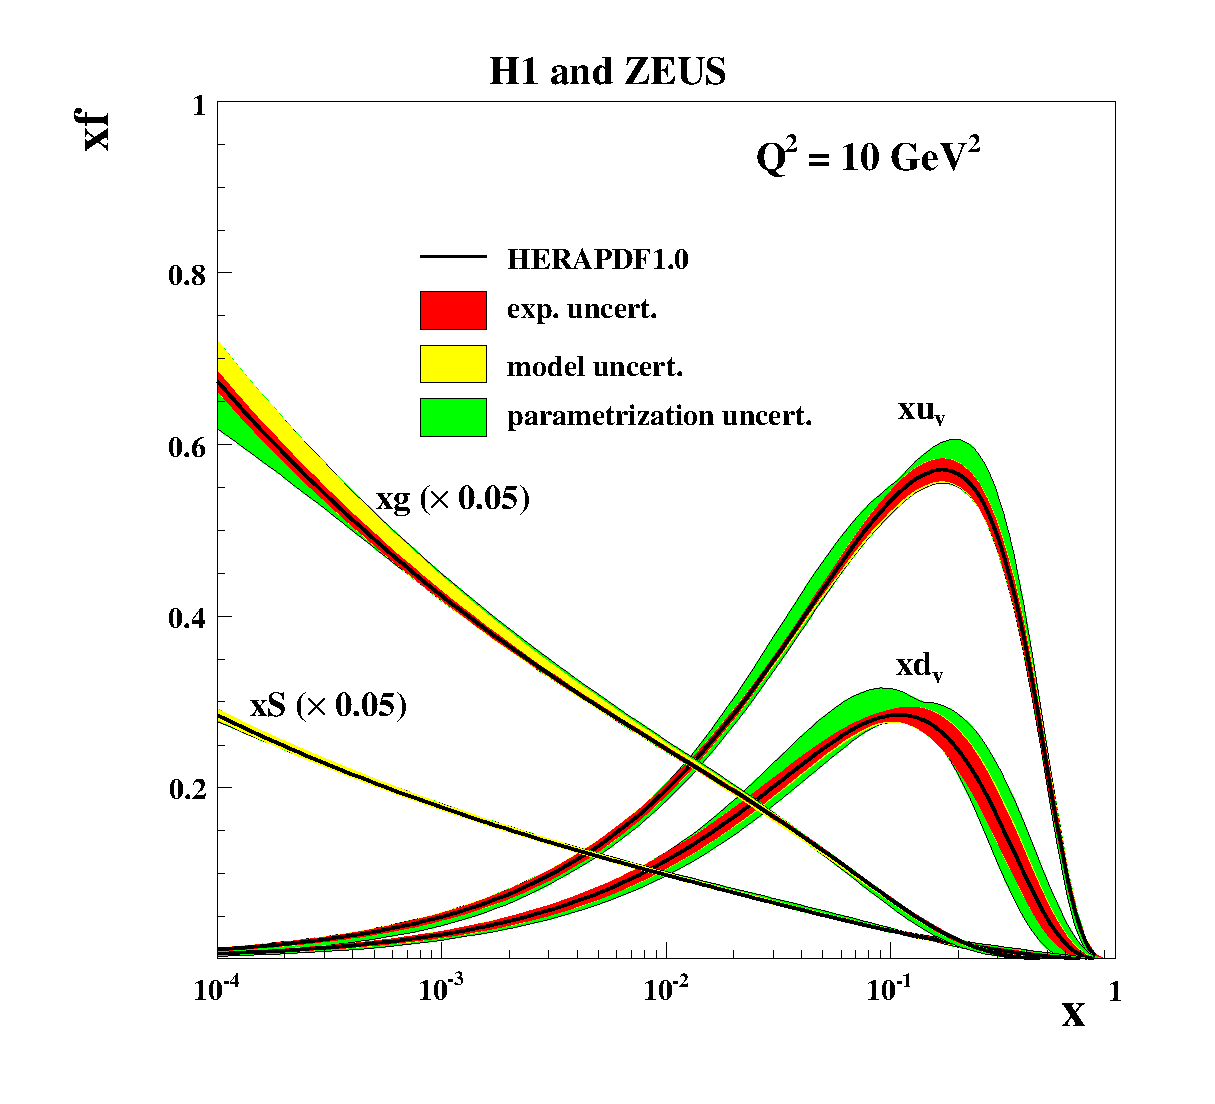
\includegraphics[width=.5\textwidth]{MCobj/d09-158f18b}
					\caption{\label{fig:HERAPDF} PDF from \textsc{HERAPDF1.0}, for up and down valence quarks $xu_v$ and $xd_v$ , gluons $xg$, and sea quarks $xS = 2x(\bar{U} + \bar{D})$, using a momentum transfer of $Q^2 =10 \GeV^2$ (from~\cite{Aaron:2009aa}).}
				\end{figure}

			\paragraph*{Matrix Element}
			%\label{sec:ME}

				The matrix element is a simulation stage used to compute the hard processes, where a large momentum transfer ($Q^2 > \mathcal{O}(1 \GeV)$) is involved, which can be calculated using quantum field theory techniques. Matrix elements to \ac{LO} or \ac{NLO} in an expansion in $\alpha_s$, to calculate a probabilistic distribution of the outgoing partons, are used to make \ac{PDFs} simulate partons coming into the hard scatter process. Hard emissions, namely the production of high momentum quarks and gluons in the event, therefore procceses such as, a gluon splitting into two gluons, $g \to gg$, or a gluon decaying to a quark-antiquark pair $g \to \qqbar$, and a quark radiating a gluon ($q \to gq$), can be added into the matrix element.

			\paragraph*{Parton Showers}
			%\label{sec:PS}

				The emission of extra soft objects cannot be modelled with the matrix element, due to its non-perturbative nature. \ac{PS} generators are instead used to include processes such as the emission of a gluon by a quark ($q \to qg$), or the emission of \qqbar\ pairs $g \to qq$ or a gluon pair by a gluon $g \to gg$. \textsc{Herwig}~\cite{Herwig2001}, \textsc{Pythia}~\cite{Pythia2006}, and \textsc{Sherpa}~\cite{Sherpa} collaborations have developed the most used \ac{PS} models across the \ac{ATLAS} community and beyond. Markov chains~\cite{Berg2004} are the heart of the algorithms used to simulate \ac{PS}. These use probabilities that a gluon is radiated or a \qqbar\ pair is produced. %The decision of whether or not these processes will occur is made at each point in the chain. 

				At intermediate $Q^2$, gluon/quark radiation may be treated as a hard emission or part of the \ac{PS}, meaning that, in a given event double-counting might occur. To overcome such issue, the \ac{CKKW}~\cite{QCD2001}, and the \ac{MLM}~\cite{ME2001}, schemes are employed to determine whether the emissions are part of the matrix element or \ac{PS}. As the energy of the partons decrease below $1 \GeV$ they will undergo hadronisation.

			\paragraph*{Hadronisation}
			%\label{sec:hadronisation}

				As previously mentioned in Section~\ref{sec:SMov}, once the quarks and gluons in the final state reach a $Q^2$ of the order of $\Lambda_{\mathrm{QCD}} \sim 200 \MeV$, the recombination into colourless objects must occur. The modelling of the production of such bound state, the hadronisation, involves non-perturbative \ac{QCD} and many more parameters than the parton showering. Phenomenological models, tuned using data, are then needed. The cluster model~\cite{ClusterHerwig1999}, used by \textsc{Herwig}, and the Lund string model~\cite{LundModel2002}, used by \textsc{Pythia}, are the most employed. 

			\paragraph*{Underlying Event}
			%\label{sec:UE}

				Partons not involved in the hard process of the event, referred to as the \ac{UE}~\cite{Field2008}, can lead to a certain number of soft interactions at a lower energy scale, therefore producing additional hadronic activity in the event. Once again, phenomenological models are used to account for such effect which is modelled within \textsc{Sherpa} and \textsc{Pythia} where a whole lot of additional free tuned-to-data parameters are included. More details can be found in~\cite{Field2008}.



		\subsection{Detector simulation}
		\label{subsec:detSim}

			Although at this stage the output of the \ac{MC} generators contains all the kinematic features of the event, it is not yet possible to compare to the \ac{ATLAS} collected data, as the interactions of the particles passing through the detectors are not yet included. The \textsc{Geant4} software~\cite{Geant42003}, included within the \ac{ATLAS} offline software\footnote{All the software made available for analysers to be used after the data have been collected}, is used to simulate the energy deposited within the detector: a first stage is run to simulate the interactions of the particles with the various sub-systems, and a second one is run to convert energy deposits into detector-output-like signals (voltage, times, etc.). This is the so-called \emph{digitisation}. The ouput is now produced with a format that is identical to the one produced by the \ac{ATLAS} \ac{TDAQ} system, therefore \ac{MC} and collected \ac{ATLAS} data can now be consistently processed by the same trigger and reconstruction softwares. Nonetheless, the \ac{ATLAS} Collaboration also use faster simulation software such as \textsc{Atlfast-II} (AF2)~\cite{Lukas2012} where, in order to reduce the usage of the available computational resources, a parametrised description of the showers in the calorimeters is implemented. 


	\section{Object Reconstruction}
	\label{sec:objReco}

		At this stage both \ac{MC} and data samples contain all the electronic pulses from the digitisation process. These have to be turned into tracks and calorimeter deposits which, in turn, have to processed to be reconstructed into physics object, such as electrons, photons, muons, jets, taus, and missing energy, \met. Initally, a set of loose definitions is employed in order for various analyses to use such objects. Later, a set of tighter cuts can be applied depending on what a particular analysis needs to focus on. This approach increases the purity of the selected objects at the expense of selection efficiency. The criteria used to define the physics objects, relevant to the analysis presented in this thesis, will be presented in the following paragraphs.


		\paragraph*{Tracks and vertices}

			When a charged particle passes through the detector, all the \ac{ID} sub-systems, pixel, \ac{SCT} and \ac{TRT} components, register ``hits''and then, tracing the particle's trajectory, the hits are reconstructed into a ``track''. The most used algorithm is the so-called \emph{inside-out} method, whose clue is in the name: it works outwards from the center of the \ac{ID} to produce a track once it has initially grouped together hits in the pixel and \ac{SCT} sub-systems. If this track is then compatible with hits in the \ac{TRT} detector, then these hits are also included and the track is accepted. The back-tracking algorithm uses the same approach, but in the opposite order, working from the \ac{TRT} to the \ac{SCT} and Pixel detectors, and tracks can also be reconstructed using only the hits in the \ac{TRT}. 

			% The ID tracks are then matched up with candidates for charged particles produced from signals in other parts of the detector, for example the ECAL cluster for an electron. A number of selection cuts are made on the tracks before this stage to ensure that they are of the required quality. The tracks are assigned values of η and φ using their direction with respect to the origin in the right-handed co-ordinate system described in Section 3.3. The origin is taken to be the position of the primary interaction, as discussed in Section 4.1. In addition, d0 is defined as the distance of closest approach between the track and the origin, and z0 is defined as the z-plane component of d0. The parameter z0 sin θ gives the projection of d0 onto the z-axis, and is also used. The transverse momentum pT of a track is related to the magnetic field B, and the bending radius R, which quantifies the bending of the track trajectory due to B. The relationship is given as pT (GeV)= 0.3×B (T)×R (m). The following cuts are applied to all tracks referred to after this point, unless otherwise specified:


		\paragraph*{Electrons}

		\paragraph*{Muons}

		\paragraph*{Photons}

		\paragraph*{Jets}

		\paragraph*{Missing Transverse Energy}

			 



	\section{Object Selection}
	\label{sec:objSel}

		\subsection{Baseline Object Selection}
		\label{subsec:baseObjSel}

			\paragraph*{Leptons}
			
			\paragraph*{Photons}
			
			\paragraph*{Jets}


		\subsection{Overlap Removal}
		\label{subsec:OR}

		\subsection{Signal Object Selection}
		\label{subsec:sigObjSel}

			\paragraph*{Leptons}

			\paragraph*{Photons}

			\paragraph*{Jets}